\chapter{Selección de eventos}\label{cap:seleccion}


Como se describe en {\XXX} las regiones de señal son un componente clave del
análisis.
En este capitulo se describe la selección de eventos que definen las regiones de
señal, que fueron optimizadas en base a la signifícanos esperada de
descubrimiento utilizando las muestras MC de señal y fondos del SM.



\section{Criterios de calidad}

%% % GRL: data12_8TeV.periodAllYear_DetStatus-v61-pro14-02_DQDefects-00-01-00_PHYS_StandardGRL_All_Good.xml

En esta análisis se ha utilizado una
GRL\footnote{\texttt{data12\_8TeV.periodAllYear\_DetStatus-v61-pro14-02\_DQDefects-00-01-00\_PHYS\_StandardGRL\_All\_Good.xml}}
que, además de aplicar requerimientos generales sobre la operación del
experimento y la estabilidad del haz en el acelerador, contiene aquellos eventos
donde todos los sub-detectores se encontraban funcionando en su plena capacidad.

Adicionalmente se eliminan los eventos que contengan algún tipo de problema,
como ruido en el calorímetro LAr, o celdas no operativas, que pueda resultar
en energía faltante instrumental. %% debido a alguno de estos problemas.



\section{Trigger}\label{sec:trigger}

Los datos fueron colectados utilizando un trigger de un fotón (\trigchain), que
selecciona eventos con al menos un fotón loose con momento transverso mayor a
120 \gev.

La eficiencia de este trigger fue calculada utilizando el método bootstrap
siguiendo las prescripciones descriptas en \cref{Damazio:1609629} y es de
$100^{+0}_{-1.41}\stat \, {}^{+0}_{-0.7}\syst \%$, con respecto a candidatos a
fotones aislados con $\pt>125 \gev$.
En la \cref{fig:trigger_perf} s se puede ver el resultado como función del {\pt}
y $\eta$ del fotón. \note{Buscar referencia y eta plot}

\begin{figure}[!htbp]
  \centering
  \includegraphics[width=0.45\textwidth]{figures/EffPtg120_loose}
  \includegraphics[width=0.45\textwidth]{figures/EffPtg120_loose}
  \caption{Eficiencia del trigger {\trigchain} como función del {\pt} (izquierda)
    y $\eta$ (derecha) del fotón.}
  \label{fig:trigger_perf}
\end{figure}

A pesar de la escasa estadística, es claro que la eficiencia alcanza una meseta,
en la cual la eficiencia es máxima, antes de $125 \gev$. La incerteza total
tiene en cuenta la limitada estadística de la muestra de datos y también la
incerteza en la corrección debido a la pureza de los fotones. El desempeño del
trigger se mantuvo estable durante todo el periodo de la toma de datos
considerado.



\section{Preselección}\label{sec:base_seleccion}

\subsection{Vertice Primario}

Como se describe en \XXX\ los candidatos a vértices de la interacción $pp$ son
reconstruidos en cada eventos utilizando las trazas en el detector interno. El
vértice primario, correspondiente a la interacción dura de dispersión, es el
candidato con la mayor suma de $p_{T}^{2}$ para las trazas asociadas. Solo se
consideran los eventos donde el vértice primario tiene al menos cinco trazas
cargadas. \note{Por que?}



\subsection{Objetos}

%% Antes de aplicar los cortes cinemáticos, se realiza la siguiente
%% preselección y limpieza.

Primero se realiza una preselección de los objetos que se consideran en cada
eventos como se detalla a continuación y en la \cref{tab:base_sel}. Se
consideran fotones a todos aquellos candidatos a fotón que pasen el criterio de
identificación \emph{tight}, que tengan $\pt>75\gev$ y $|\eta|<2.37$. Se
consideran electrones que pasan el criterio de identificación \emph{medium}, y
que tengan un $\pt>10\gev$ y $|\eta|<2.47$, y muones que pasan un criterio de
identificación \emph{loose} con $\pt>6 \gev$ y $|\eta|<2.5$. Para el caso de
jets, se consideran los que tienen $\pt>20\gev$ y $|\eta|<2.8$.


\begin{table}[ht!]
  \centering

  \caption{Preselección de objetos. Criterio de identificación (ID), y cortes de
    aceptancia (\pt, $\eta$) considerados para cada tipo de partícula. Además
    del limite superior en $|\eta|$, no se consideran en ningún caso los objetos
    que se encuentren en la zona entre la zona central y las tapas del detector, es
    decir, con $1.37 < |\eta| < 1.52$.}
  \label{tab:base_sel}

  \begin{tabular}{p{0.2\textwidth}x{0.2\textwidth}x{0.2\textwidth}x{0.2\textwidth}}
    \hline
    & ID & $\pt$ & $|\eta|$ \\
    \hline
    Fotones    & \emph{tight}  & $> 75 \gev$ & $<2.37$ \\
    Electrones & \emph{medium} & $> 10 \gev$ & $<2.47$ \\
    Muones     & \emph{loose}  & $> 6  \gev$ & $<2.5$  \\
    Jets       & -             & $> 20 \gev$ & $<2.8$  \\
    \hline
  \end{tabular}

\end{table}


%% La selección de los objetos se realiza según lo descripto en \cref{sec:obj_selection}.
%% El overlap removal y el event veto aplicado se detalla en la \cref{sec:overlap_romoval_event_veto}.

%% Excepto durante calculo de {\met}, dos cortes de aceptancia extra son requeridos
%% para los jets: $\pt > 40 \gev$ y $|\eta| < 2.8$.
%% Todos los jets pasando esta selección \emph{loose} son considerados cuando se aplica
%% la identificación de objetos descripta en \cref{sec:overlap_romoval_event_veto}.


\subsection{Eliminación de objetos superpuestos} %% y veto de eventos\note{?}}
\label{sec:overlap_romoval_event_veto}

De acuerdo a las definiciones de objetos anteriores, un objeto puede estar en
mas de una categoría, contándose dos veces. Por este motivo se realiza un
procedimiento para remover este solapamiento, el cual se aplica sobre los
objetos preseleccionados antes de aplicar los criterios de aislamiento. El
procedimiento para remover estas ambigüedades entre los objetos es el que se
detalla a continuación en ese orden:

\begin{itemize}\itemsep0.1cm
\item Si un fotón o electrón se encuentran dentro de $\Delta R < 0.01$, el
  objeto es considerado como un electrón, removiéndose el fotón correspondiente.
  Esta elección reduce la taza de electrones mal reconstruidos como fotones.
\item Los jets que estén cerca ($\Delta R<0.2$) de un electrón o fotón
  preseleccionado se remueven.
\item Fotones y electrones preseleccionados son removidos si su distancia al jet
  mas cercano es $0.2 < \Delta R < 0.4$.
\item Muones preseleccionados son removidos si su distancia al jet más cercano
  es $\Delta R < 0.4$.
\end{itemize}


\subsection{Limpieza de eventos}

Para asegurar el correcto calculo de la energia faltante, y eliminar
los eventos con energia faltante instrumental, los eventos que satisfacen
alguna de las condiciones siguientes son descartados.

\begin{itemize}\itemsep0.1cm
\item Si el evento (después de de la preseleccion de objetos y la eliminacion de los objetos superpuestos) contiene al menos
  un jet que falla los cortes de limpieza de jets que se definen en
  \cref{sec:jet_obj}.

\item Eventos con muones cósmicos: cuando el evento tiene al menos un muon con $|z_{0}| > \unit[1]{mm}$ o $|d_0| >
  \unit[0.2]{mm}$, donde estos valores son calculados con respecto al vértice
  primario. %%Estos muones tienen altas posibilidades de ser muones cosmicos \note{Check!}
\end{itemize}

Después de esta limpieza de eventos, con los objetos definidos en las secciones anteriores y después
de haber eliminado los objetos duplicados, se calcula la energía faltante transversa como se explica
en \cref{sec:met_obj}.



\section{Optimización de las regiones de señal}

Después de la preselección descripta en las secciones anteriores, es necesario
definir las regiones de señal, es decir, las regiones enriquecidas en eventos
de señal en las cual se realizara el experimento de conteo.
 Definir una región de señal implica la definición de una selección (un conjunto
 de cortes) en ciertos observables.


Como primer paso se seleccionan eventos que contengan el estado final buscado:
un fotón, y energía faltante. Y a partir de eso se buscan observables que
permitan separar la señal del fondo y se optimizan los cortes en estos observables.
%Adicionalmente, se imponen algunos cortes para ``limpiar'' el evento de posibles


%% la selección final que se aplicara a los
%% eventos, que deberá estar enriquecida en eventos de señal y tener un alto
%% rechazo a eventos de fondo. Para lograr este objetivo se optimiza la selección
%% haciendo uso de las muestras simuladas con MC tanto para señal como para los
%% procesos del SM.

Del estudio realizado en la sección {\XXX}, resulta evidente las diferencias
cinemáticas y topológicas de los eventos en las distintas regiones del
espacio de parámetros {\mgmn} del modelo de SUSY.
Es por esta razón que resulta conveniente tener mas de una región de señal,
cada una destinada a una zona particular de la grid de señal.

%% que lo mas conveniente es
%% definir dos regiones de señal, cada una de ellas optimizada para las dos
%% regiones claramente distintas en cuanto a sus características cinemáticas y
%% topológicas.

Por tal motivo, se dividió el análisis en dos regiones de señal, a las que se
llamó {\SRL} y {\SRH}.
La primera región de señal, \SRL, dirigida a la zona de gluinos de alta masa que
decaen en cascada hasta neutralinos NLSP de baja y moderada masa. Los eventos de
señal en esta región se caracterizan por un gran multiplicad de jets y actividad
hadronica, debido a que involucra cadenas de decaimiento largas de gluinos
pesados a través de producción de charginos. Cuanto mas baja la masa del
{\ninoone}, más baja sera la energía del fotón y menor es la cantidad de
energía faltante.
La segunda región de señal, \SRH, tiene como motivación los escenarios donde la
masa del gluino y del neutralino mas liviano están cerca una de la otra. La
cadena de decaimiento es por lo tanto mucho mas corta en este caso, con una
menor multiplicidad de jets, y debido al neutralino pesado, fotones de alto
{\pt} y gran cantidad de energía faltante en el estado final.

En la \cref{fig:srs_motivation} puede ver esquemáticamente a que región del espacio
del parámetros de la señal \mgmn esta destinada cada SR.

\begin{figure}[!htbp]
  \centering
    \resizebox{0.5\textwidth}{!}{
      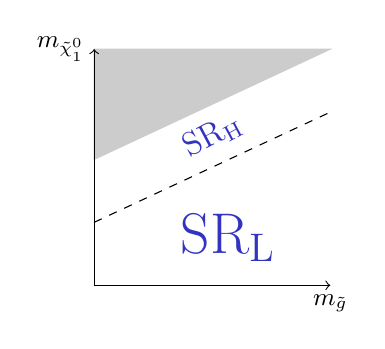
\begin{tikzpicture}

  \colorlet{green}{green!50!black!50}
  \colorlet{red}{red!70!black!50}
  \colorlet{blue}{blue!70!black!80}

  \draw[gray!40,fill] (0, 1.6) -- (3, 3) -- (0,3) -- cycle;

  \draw[->] (0,0) -- (3,0) node[below] {\small $m_{\tilde{g}}$};
  \draw[->] (0,0) -- (0,3) node[left] {\small $m_{\tilde{\chi}_1^0}$};

  %\draw[red,line width=2] (1.5,1.8) circle (15pt);
  \draw[dashed] (0,0.8) -- (3, 2.2);

  \node[blue] at (1.7,0.6) {\huge SR$_{\mathrm{L}}$};
  \node[blue] at (1.5,1.9) [rotate=28] {\large SR$_{\mathrm{H}}$};

\end{tikzpicture}

      }
    \caption{Esquema de la región del espacio de parámetros del modelo de señal en el
    plano {\mgmn} y a que zona esta dirigido el diseño de las dos regiones de señal.}
  \label{fig:srs_motivation}
\end{figure}


Para la optimización de las SR, se utilizaron varios puntos de señal en cada región,
representativos de la topología y el espacio de fase en cada caso.

\begin{itemize}\itemsep0.2cm\parskip0.2cm
\item {\SRL}: (1150, 175) y (1150, 450)
\item {\SRH}: (1150, 850) y (1150, 1050)
\end{itemize}


Se utilizaron los fondos MC, y se considero una incerteza en la estimación del
fondo de 25\%. Todas las muestras MC fueron normalizadas a una luminosidad total
integrada de $20.3 \ifb$. La significancia esperada se calculo utilizando la
\cref{eq:Za}, y para evitar una selección muy restringida, se requiere al menos
un evento de fondo en cada SR. Además de evaluar la significancia esperada para
distintos cortes también se tuvo en cuenta que la eficiencia de señal no sea
menor a 20\%.

Los cortes fueron optimizados en el orden de poder discriminatorio, uno a la
vez, y aplicados en el orden descripto a continuación, monitoreando la
significancia para distintos cortes en las variables discriminatorias.

Como ya se ha mencionado el estado final buscado en este análisis consiste en un
único fotón, jets y energía faltante. Por lo que la definición de las SR
comienza optimizando los cortes en las variables cinemáticas del fotón, los jets
y el corte en energía faltante.

%% Como primer paso se impuso un corte en la energia faltante transversa $\met>150\gev$Se impuso
%% La significancia para cada caso
%% The significance for different cut combinations was also monitored to take the best configuration.
%% A minimal pre-selection cut in $\met>150\gev$ was placed in the SR, which is highly efficient for the signal and very effective
%% removing large part of the SM backgrounds, particularly the QCD multijet production. The final selection requirements are summarised in sec \ref{sec:signal_regions}.



%% \begin{figure}[h!]
%%   \centering
%%   \includegraphics[width=0.5\textwidth]{figures/grid_regions.pdf}
%%   \caption{Regiones de senal usadas en este analisis.
%%     Los cuadrados azules corresponden a cada muestra de senal simulada en la
%%     grid \M{3}-$\mu$.
%%     El área gris es una región cismáticamente prohibida ($m_{\gluino}<m_{\ninoone}$).}\label{fig:SRegions}
%% \end{figure}


\subsection{Fotón}\label{sec:opt_ph_iso}

El primer paso para definir la SR consistió en seleccionar eventos con un único
fotón de los previamente seleccionados con {\pt} mayor a 125 \gev. Este valor se
eligió para que esté por encima de la meseta de la eficiencia del trigger. En la
\cref{fig:photon_pt} se muestra las distribuciones del {\pt} del fotón para los
eventos de fondo del {\SM} como también para algunos puntos de señal.

Los eventos con un segundo fotón con $\pt > 75 \gev$ fueron vetados. El corte en {\pt}
 de $75\gev$ fue elegido para que las SR sean ortogonales a las SR del análisis de ATLAS
que busca dos fotones\cite{ATLAS-CONF-2014-001}
y la posible combinación estadística con el mismo. Este otro análisis fue diseñado
para buscar SUSY en escenarios GGM, pero particularmente en el caso de que el
neutralino NLSP sea mayoritariamente bino, y el decaimiento a fotones sea
dominante.


%% \begin{figure}[!htbp]
%%   \centering
%%   \includegraphics[width=0.45\textwidth]{figures/ph_pt_base1}
%%   \includegraphics[width=0.45\textwidth]{figures/ph_pt_base2}
%%   \caption{Distribución del {\pt} del fotón para señal y fondo MC en {\SRL} (izquierda) y
%%     {\SRH} (derecha), correspondiente a una luminosidad integrada de {\ilumi} antes de que ningún
%%     corte haya sido aplicado. }
%%   \label{fig:photon_pt}
%% \end{figure}

Como se menciona en la \cref{sec:pho_obj}, para seleccionar los fotones se
aplica un corte en la energía transversa de aislamiento. Se estudiaron distintos
criterios de aislamiento, en los que varia el tamaño del cono ($R$) en el cual se
calcula esta energía.

%% La optimización de este criterio de aislamiento  fue realizada mirando el desempe\~no
%% de los distintos tamaños de cono.

En la \cref{fig:photon_iso} se muestra las distribuciones de la energía de
aislamiento para varios valores de $R$ para las muestras de señal en las dos SR.
La SR con mayor diferencia de masa entre gluino y neutralino parece tener
distribuciones mas anchas, un efecto que desaparece para tamaños de cono mas
chicos. Como se ve en la \cref{fig:photon_iso_sig} (arriba), la mayor eficiencia
de selección se obtiene también para el menor tamaño de cono, $R = 0.2$. Para un
corte de $5 \GeV$, obtenemos una eficiencia alta (85-90\%) a lo largo de toda la
grid. Luego de aplicar una preselección en {\met}, los fotones no aislados
provenientes de fondos procesos QCD son muy suprimidos, reduciendo el impacto
del corte de aislamiento en la significancia.

Incluso luego de que la corrección es aplicada para remover la filtración de
energía del fotón dentro de su propio cono de aislamiento, una dependencia reman
te con el {\pt} del fotón es observada para todos los tamaños de cono
considerados, como se muestra en \cref{fig:photon_iso} (abajo). El tratamiento
de este efecto es discutido en la \cref{sec:jfake_sig_template,sec:expsyst}.


\begin{figure}[!htbp]

  \centering
  \includegraphics[width=0.32\textwidth]{figures/iso_20}
  \includegraphics[width=0.32\textwidth]{figures/iso_30}
  \includegraphics[width=0.32\textwidth]{figures/iso_40}

  \includegraphics[width=0.32\textwidth]{figures/iso_20_pt}
  \includegraphics[width=0.32\textwidth]{figures/iso_30_pt}
  \includegraphics[width=0.32\textwidth]{figures/iso_40_pt}

  \caption{Distribución de {\etiso} (arriba) y su promedio como función del
    {\pt} del fotón (abajo) para distintos tamaños de conos: $R=0.2$, $R=0.3$ y$R=0.4$.
    Una preselección de $\pt>120\gev$ y $\met>150\gev$ fue aplicada.}
  \label{fig:photon_iso}
\end{figure}

\begin{figure}[!htbp]
  \centering

  \includegraphics[width=0.3\textwidth]{figures/iso_20_sig}
  \includegraphics[width=0.3\textwidth]{figures/iso_30_sig}
  \includegraphics[width=0.3\textwidth]{figures/iso_40_sig}

  \includegraphics[width=0.3\textwidth]{figures/iso_20_eff}
  \includegraphics[width=0.3\textwidth]{figures/iso_30_eff}
  \includegraphics[width=0.3\textwidth]{figures/iso_40_eff}

  \caption{Significancia (arriba) y eficiencia (abajo) vs. el corte en la energía de
    aislamiento, después del corte en {\pt} y {\met}.}
  \label{fig:photon_iso_sig}
\end{figure}



\subsection{Leptones}\label{sec:leptonphoton_veto}

Además del veto a los eventos con un segundo fotón, también se remueven
los eventos que contienen leptones ($e$ o $\mu$) con el objetivo de que las
SR no tengan un solapamiento con las SR del análisis que busca un fotón, un
leptón y energía faltante\note{cite?}. La disminución en la eficiencia
debido a este veto es de XXX \%.



\subsection{Energía faltante}

La principal característica de los eventos de SUSY donde se conserva
la paridad-R, es la presencia de una gran cantidad de energía faltante.
Un corte en esta variable reduce enormemente la contaminación de procesos
QCD y también de otros procesos del {\SM}.
La \cref{fig:opt_met} muestra la distribución de {\met} en eventos con
un fotón aislado con alto {\pt} (como se definió en la sección anterior),
para dos puntos de señal en cada SR, junto al fondo esperado de simulaciones
MC.

Un corte en {\met} relativamente bajo ($> 200 \gev$) es capaz de separar
la señal y el fondo significativamente en {\SRL}, mientras que para {\SRH}
es posible aplicar un corte más alto ($>300\gev$).

\begin{figure}[!htbp]
  \centering
  \includegraphics[width=0.49\textwidth]{met_et_base1}
  \includegraphics[width=0.49\textwidth]{met_et_base2}
  \caption{Energía faltante transversa para una luminosidad integrada de {\ilumi}
    luego de que se aplique el corte en el {\pt} del fotón y en la energía de aislamiento
    para los puntos de señal de {\SRL} (izquierda) y {\SRH} (derecha). }
  \label{fig:opt_met}
\end{figure}



\subsection{Multiplicidad y {\pt} de los jets} \label{sec:opt_njet}

En la \cref{fig:jets_npv} se muestra, el valor medio del numero de jets
seleccionados como funcion del numero de vertices en el evento, para
distintos cortes en el {\pt} de los jets. A medida que aumenta el corte
en {\pt} el numero de jets se hace mas estable con el pile-up, y por lo
tanto en este analisis se consideran los jets con $\pt>40\gev$

%% El corte en {\pt} fue elegido para asegurar una selección robusta contra el pile-up.


\begin{figure}[!htbp]
  \centering
  \includegraphics[width=0.5\textwidth]{data_jets_npv}
  \caption{Valor medio del numero de jets vs. el número de vértices primarios
    observados en datos para distintas selecciones de $\pt^{jet}$.}
    \label{fig:jets_npv}
\end{figure}



%% Como se muestra en la \cref{fig:jets_npv}, el numero medio de jets seleccionados
%% es de esta forma una distribución \hl{flat} como función del numero de vértices
%% primarios. Luego, en la selección final, cortes mas alto en el {\pt} de los jets
%% son utilizados como se describe en \cref{sec:opt_njet}.

La \cref{fig:opt_jet_n} muestra la multiplicidad de jets ($N_{\mathrm{jet}}$) para
$\pt^{\mathrm{jet}} > 40$ \gev, después de los cortes optimizados en el fotón y la {\met}
descriptos anteriormente.
Mientras que la señal tiene típicamente un gran número
de jets, la mayoría de los fondos W/Z+jets, diboson y QCD se acumulan en la zona
de pocos jets. Al menos dos (cuatro) jets son requeridos para los eventos que
pasa la selección de {\SRL} ({\SRH}).
Una mayor multiplicidad es efectivamente
esperada para {\SRL} debido a que su objetivo es la región de gluinos pesados
donde el decaimiento dominante es el de producción de cárganos por un
decaimiento de tres cuerpos.

\begin{figure}[!htbp]
  \centering
  \includegraphics[width=0.49\textwidth]{jet_n_base1}
  \includegraphics[width=0.49\textwidth]{jet_n_base2}
  \caption{Número de jets en la {\SRL} (izquierda) y {\SRH} (derecha) con $\pt > 40 \gev$,
    después de la seleccion en el {\pt} del fotón y $\met > 150\gev$, para una luminosidad integrada de {\ilumi}.}
  \label{fig:opt_jet_n}
\end{figure}

%{\fig} \ref{fig:jetlead_3SR}  shows the \pt\ of the leading jet, after the photon \pt\ and \etmiss cut,
%and requiring the number of jets to be equal or larger than two for SR1-SR3, and equal or larger than
%four for SR2. Additional signal-background discrimination can be obtained by imposing cuts on the %leading
%jet \pt\ (\pt$(j1)$)since the signal tends to have hard leading jets, in particular for the case involving large
%gluino masses and low to medium neutralino masses (SR2).  For SR1 and SR2 the leading jet \pt\  is %required
%to be larger than 80 \gev~ and 100 \gev, respectively.   After those cuts, in  {\fig} \ref{fig:jetsublead_3SR},
%the subleading jet \pt\  (\pt$(j2)$) distributions for the three signal regions are shown. A further cut is %applied for
%SR1 and SR2, by requiring $\pt(j2)>80$ \gev~  and $> 100$ \gev, respectively.

%% La \cref{fig:opt_jet_p1} muestra el {\pt} del jet mas energético ($\pt^{j1}$),
%% después de los cortes descriptos anteriormente. %Adicionalmenteafter the
%% photon \pt, \etmiss\ and $N_{jet}$ requirements described above for each signal region.

En la {\SRL} es posible obtener una disccriminacion requiriendo ademas que los dos jets
mas energeticos tengan $\pt>100 \gev$.
%% En la {\SRH} donde la masa del gluino y la NLSP
%% es menor, een
%% Additional signal-background discrimination can be achieved by requiring a hard leading
%% jet, particularly for SR2 where the heavy gluinos decay down to relatively light neutralinos.
%% Thus, the leading jet \pt\ in SR2 is required to be larger than 100 \gev. Although a
%% harder requirement is suggested by {\fig} \ref{fig:jetlead_3SR}, it was found better to
%% keep it relatively loose and rely on the shape variables described in sec \ref{sec:shape_vars}.
%% The smaller mass difference between gluino and the lightest neutralino in SR3 leads to a
%% softer jet spectrum and then no further requirement is applied in this region.
%Additional signal-background discrimination can be obtained by imposing cuts on the leading  jet \pt\ since the signal tends to have hard leading jets, in particular for the case involving  large gluino masses and low to medium neutralino masses (SR2).  For SR1 and SR2 the leading jet \pt\  is required to be larger than 80 \gev~ and 100 \gev, respectively.

%% \begin{figure}[!htbp]
%%   \centering
%%   \includegraphics[width=0.49\textwidth]{figures/figura} %jet1_pt_SR2}
%%   \includegraphics[width=0.49\textwidth]{figures/figura} %jet1_pt_SR3}
%%   \caption{Momento transverso del jet mas energético en {\SRL} (izquierda) y {\SRH} (derecha),
%%     para una luminosidad integrada de {\ilumi}.}
%%   \label{fig:opt_jet_pt1}
%% \end{figure}

%% A continuacion se exploro el momento transverso del segundo jet mas energetico ($\pt^{j2}$).
%% Las distirbuciones para cada region pueden verse en \cref{fig:opt_jet_pt2}. En {\SRL}
%% se encontro que un corte en $\pt^{j2}>100$ \gev

%% \begin{figure}[!htbp]
%%  \centering
%%  \includegraphics[width=0.49\textwidth]{figures/figura} %jet2_pt_SR2}
%%  \includegraphics[width=0.49\textwidth]{figures/figura} %jet2_pt_SR3}
%%   \caption{Momento transverso del segundo jet mas energético en {\SRL} (izquierda) y {\SRH} (derecha),
%%     para una luminosidad integrada de {\ilumi}.}
%%  \label{fig:opt_jet_pt2}
%% \end{figure}



\subsection{Ángulo entre jets y \met}
\label{sec:dphi_obj}

En los eventos de señal, la energía faltante es producida por los dos
gravitinos. Se espera por lo tanto que la dirección del {\met} sea aleatoria,
sin estar correlacionada con ninguno de los demás objetos del evento. Por otro
lado, si la {\met} es originada de efectos instrumentales o de neutrinos
energéticos en $b$-jets o $c$-jets, la dirección del {\met} estará
correlacionada con uno de los jets mal medidos. La
\cref{fig:jet_jet-MET-phi_3SR} muestra el mínimo $\Delta\phi$ entre la dirección
de {\met} y la de los dos jets mas energéticos.

%% \begin{equation} \label{eq:dphi}
%%   %%\min\left[ \cos   \Delta\phi({\rm jet}_{1,2},\MET) \right] \equiv  \min \left[\frac{\vec{\met} \cdot \vec{p}_{\rm T}^{\rm \; jet,i}}{|\vec{\met}|  |\pt^{\mathrm{jet},i}|}\right] \quad \quad i = 1,2
%%   \cos \Delta\phi(\mathrm{jet},\met) \equiv \frac{\vec{\met} \cdot \vec{p}_\mathrm{T}^{\mathrm{jet}}}{|\vec{\met}| |\pt^{\mathrm{jet}}|}
%% \end{equation}
%% %

%% after applying the photon \pt, \met, jet {\pt} and multiplicity cuts.
%% A lower bound $\dphijm>0.4$ cut is applied for the two signal regions,
%% which helps to significantly reduce the QCD background and clean events with mis-reconstructed \etmiss.

\begin{figure}[!htbp]
  \centering
  \includegraphics[width=0.49\textwidth]{figures/dphi_jetmet_srl}
  \includegraphics[width=0.49\textwidth]{figures/dphi_jetmet_srh}
  \caption{$\Delta \phi \text{(jet, \MET)}$ para {\SRL} (izquierda) y {\SRH} (derecha)}
  \label{fig:jet-MET-phi_3SR}
\end{figure}


\subsection{Ángulo entre jet y fotón}

Para regiones del espacio de parámetros del modelo de señal
donde los gluinos y los neutralinos tienen alta masa ({\SRH})
un corte en la separación entre el fotón y los jets ayuda a
reducir el fondo, principalmente proveniente de dijets y
fotones directos, donde un fotón (real o falso) tiende a ser
producido en la dirección opuesta al jet mas energético.
%% El ángulo azimutal entre el fotón y el jet principal se define
%% como:

%% \begin{equation} \label{eq:dphi}
%%   \cos \dphijg \equiv \frac{\vec{p}_\mathrm{T}^{\gamma} \cdot \vec{p}_\mathrm{T}^\mathrm{jet}}{|{p}_\mathrm{T}^{\gamma}| |\pt^\mathrm{jet}|}
%% \end{equation}

%
%% which distribution is shown in {\fig} \ref{fig:jet-photon-phi_SR3},
%% for {\SRH} benchmark signal samples after all previous selection.
%% The cut value chosen for this high gluino-neutralino mass region is $\dphijg<2$.

 % shows the jet-photon $\phi$ separation for signal and backround in SR3, after applying the photon \pt\ ,  \etmiss,  jet  \pt\  and multiplicity as well as  $\Delta \phi \text{(jet, MET)}$ cuts.  The cut value chosen for jet-photon separation in this high mass signal region  is  $\Delta \phi \text{(jet}, \gamma) >2$.
%%   \begin{figure*}[th!]
%%  \centering
%%    \includegraphics[width=0.49\textwidth]{figures/figura}
%%    \caption{\dphijg\ for {\SRH}, after applying the photon \pt, \met, jet multiplicity, jet \pt\ and \dphijm\ cuts
%%      (See text for details), for an integrated luminosity of 20.3 \ifb.  For illustration,
%%    distributions for three signal points are also shown.}
%% \label{fig:jet-photon-phi_SR3}
%% \end{figure*}


\subsection{Energia Total Transversa (\HT)}
\label{sec:ht_obj}

Dada la gran masa de los gluinos producidos en las colisiones, en el espacio de
parámetros explorado en este análisis, se espera que la energía transversa
visible total sea alta. Por eso, el observable {\HT} definido como la suma
escalar de la energía transversa de todos los objetos observados en el estado
final es mucho mayor para eventos de señal que para los eventos de fondo.
Después del veto a los eventos con leptones, {\HT} se define como:

\begin{equation} \label{eq:htaddition}
  \HT \equiv \pt^{\gamma} + \sum_{\mathrm{jets}} \pt^\mathrm{jet}
\end{equation}

La \cref{fig:opt_ht} muestra las distribuciones de {\HT}.
Para {\SRL}, se espera incluso que {\HT} sea mayor, debido a la
diferencia de masa entre el gluino y el neutralino NLSP. Sin embargo
se encontró una variable mas efectiva para la separación entre señal y
fondo que se describe a continuación y por lo tanto no se aplica un corte
en esta variable.

%photon \pt,  \etmiss, jet multiplicity, two leading jets  \pt,   jet-\etmiss\  and jet-photon $\phi$ separation cuts.
%A large \HT\ requirement ($>800 \gev$) helps reducing the remaining SM background in SR3. Given the high mass neutralino, the main contribution to \HT\ is coming from the hard photon in the event.
%particularly,  SR3 as significantly larger hadronic activity is observed in the signal samples.  NO
%Cuts are then applied, requiring \HT  larger than 800 \gev\  for both SRs.

\begin{figure}[!htbp]
  \centering
  \includegraphics[width=0.49\textwidth]{ht_srl} %ht_SR2}
  \includegraphics[width=0.49\textwidth]{ht_srh} %ht_SR3}
  \caption{Distribución de la energia total transversa (\HT) para {\SRL} (izquierda)
    y {\SRH} (derecha).}
    %.distributions for SR2 (left) and SR3 (right).}
    %% after photon \pt, \etmiss, jet multiplicity, jet \pt\ and angular cuts
    %% (see text for details), for an integrated luminosity of 20.3 \ifb.  For illustration,
    %% distributions for three signal points in each signal regions are also shown.}
  \label{fig:opt_ht}
\end{figure}


\subsection{Variables de forma adicionales}\label{sec:shape_vars}

Adicionalmente, muchas variables de forma fueron exploradas para poder obtener
una discriminación adicional entre señal y fondo. En especial se estudio el
observable $R_T^n$ definida como

\begin{equation}\label{eq:rt_formula}
  R_{T}^{n} = \frac{\sum_{i=1}^{n}p_\mathrm{T}^{j_i}}{\sum p_\mathrm{T}^{j}},
\end{equation}
%
es decir, el cociente entre la suma escalar de los {\pt} de $n$ jets y la suma
escalar del {\pt} de todos los jets en el evento, donde $n$ es el mínimo número
de jets requerido.

%% It is evident that the distribution pattern of this variable, as pointed
%% out in \cite{PhysRevD.84.055010}, depends on the multiplicity and hardness of the jets. As shown in previous sections, the SUSY signals here considered are characterized by hard multijet events in a wide region of parameter space. Evenmore, the sub-leading jets are comparatively harder than those in SM background events. In the case when

%% $n_{j}^{min} \sim n_{j}$, which is predominant in the latter,
%% then the numerator and denominator in {\eq} \eqref{eq:rt_formula}
%% are almost identical and hence the ratio is close to unity. For signal processes, with $n_{j}^{min} \ll n_{j}$ and comparatively harder jets, the ratio is mostly distributed way below 1.

\begin{figure}[!htbp]
  \centering

  \includegraphics[width=0.49\textwidth]{figures/rt4_srl}
  \includegraphics[width=0.49\textwidth]{figures/rt2_srh}

  \caption{Distribucion de {\rt} para {\SRL} y {\rtt} para {\SRH}}
  \label{fig:opt_rt}
\end{figure}

La \cref{fig:opt_rt} (izquierda) muestra la distribución de {\rtt} para {\SRH},
después de la selección final excepto el corte en {\rtt}. Mientras que la
\cref{fig:opt_rt} muestra la distribución de {\rt} para {\SRL}. El bajo numero
de jets para {\SRH}, hace que la distribución de {\rtt} para los eventos de
señal sea similar a la del fondo QCD, y por lo tanto el observable no es útil
para rechazas fondo manteniendo una aceptancia razonable. Para el caso de {\SRL}
un corte $\rt < 0.85$ permite reducir en una fracción considerable el fondo con
una perdida muy chica en la eficiencia de señal.



\section{Selección Final}\label{sec:signal_regions}

Como resultado del proceso de optimización descripto en la sección anterior,
se definen las dos regiones de señal:

\begin{itemize}\itemsep0.2cm
\item[{\bf {\SRL}}] dirigida a detectar eventos en los que gluinos de alta masa
  son producidos, y decaen a neutralinos de baja/media masa. Estos eventos estan
  caracterizados por objetos de alta energia? y una gran multiplicidad de jets
  energeticos.
\item[{\bf {\SRH}}] dirigida a detectar eventos en los que los gluinos
  producidos decaen en neutralinos con una masa similar. These events are
  characterized by high energy scales.
\end{itemize}

Cada región de señal queda definida por los cortes de selección detallados en la \cref{tab:final_sel_sr}.

\begin{table}[!htbp]

  \centering
  \caption{Conjunto de cortes en los observables que definen las dos regiones de señal, {\SRL} y {\SRH}.}
  \label{tab:final_sel_sr}

    \begin{tabular}{x{0.25\textwidth}x{0.25\textwidth}x{0.25\textwidth}}
    \hline
    & {\bf \SRL} & {\bf \SRH} \\
    \hline
    \# fotones & $=1$ & $=1$ \\
    \ptgam & $>125 \gev$ & $>300 \gev$ \\
    \# leptones & \multicolumn{2}{c}{$=0$} \\
    \# jets & $\geq 4$ & $\geq 2$ \\
    $\pt^{j1}$ & $>100 \gev$ & - \\
    $\pt^{j2}$ & $>100 \gev$ & - \\
    $\Delta\phi(\mathrm{jet}, \met)$ & $>0.4$ & $>0.4$ \\
    {\met} & $>200 \gev$ & $> 300 \gev$ \\
    $R_T^4$ & 0.85 & - \\
    $H_T$ & - & $>800 \gev$ \\
    $\Delta\phi(\gam,\mathrm{jet})$ & - & $<2.0$ \\
    \hline
  \end{tabular}

\end{table}




El número de eventos esperado de fondos el {\SM} de las muestras simuladas
después de la selección completa se muestran en la \cref{tab:mc_events_sr1}.
,\ref{tab:mc_events_sr2}, para {\SRL} y {\SRH}, respectivamente.
También se presenta el numero de eventos esperado y la significancia para tres puntos
de señal relevantes en cada región de señal.

Se puede ver que la contaminación dominante viene de {\wgam} y {\ttgam}. Adicionalmente
en la \cref{tab:mc_events_sr_phtype} se puede ver el numero de eventos de fondo
esperado separando fotones reales de los eventos donde un jet o un electrón es confundido
con un fotón. El primero tipo de eventos es claramente dominante en este análisis, en
presencia de energía faltante tanto real como instrumental.

La significancia esperada en la grid de señal completa se puede ver en la \cref{fig:opt_exp_significance},
incluyendo el mejor valor de ambas regiones. Es importante notar que estos
resultados son preliminares y obtenidos de simulaciones Monte Carlo. Los resultados
finales son derivados utilizando los métodos de estimación de fondos descriptos en
el \cref{cap:fondos}. %%, y luego del procedimiento descripto en nd after the fitting procedure detailed in \cref{sec:fitresults}.

\begin{table}[!htbp]
  \centering
  \caption{Número de eventos esperado para los fondos del {\SM}
    y algunos puntos de señal después de cada corte de la región
    de señal {\SRL}, para una luminosidad integrada de {\ilumi}. Para los
    puntos de senal, tambien se muestra en la ultima fila, la
    significancia esperada ($Z$).}
  \label{tab:exp_bkg_srl}

  \resizebox{\textwidth}{!}{
    \begin{tabular}{ccccccccccc}
      \hline
      {\bf \SRL}   & (1050,175) & (1150,175) & (1150,650) &  W/Z + $\gam$ & Diboson & W/Z + jets & QCD & \ttbar & \ttbar\gam & Fondo total \\
      \hline
      Un fotón                    & 3696.00 & 3671.03 & 50.52 & 29378.86 & 297.09 & 12694.40 & 3392496.25 & 344.62 & 1820.71 & $3437031.93\pm8506.93$ \\
      \ptgam                       & 3199.64 & 3177.24 & 49.51 & 25195.24 & 230.19 & 10093.10 & 2826296.25 & 251.46 & 1585.17 & $2863651.40\pm7748.67$ \\
      Veto leptones                     & 2903.73 & 2890.27 & 34.74 & 22215.54 & 166.08 & 7808.01 & 2824994.75 & 204.99 & 1084.30 & $2856473.68\pm7725.42$ \\
      N jets                           & 106.54 & 93.15 & 24.99 & 1976.64 & 15.38 & 172.66 & 82028.19 & 66.49 & 518.61 & $84777.97\pm3059.93$ \\
      $\pt^{j1}$                        & 84.70 & 71.29 & 24.85 & 1749.41 & 14.29 & 142.19 & 69374.30 & 57.86 & 427.33 & $71765.38\pm3019.91$ \\
      $\pt^{j2}$                        & 53.55 & 40.39 & 23.38 & 1066.33 & 8.71 & 95.60 & 37144.05 & 34.06 & 240.60 & $38589.36\pm708.87$ \\
      $\Delta\phi(\mathrm{jet}, \met)$  & 44.78 & 33.88 & 20.07 & 828.96 & 7.83 & 68.13 & 28194.02 & 27.88 & 184.41 & $29311.22\pm613.45$ \\
      \met                             & 14.10 & 9.44 & 15.96 & 7.00 & 0.93 & 0.00 & 2.52 & 1.83 & 4.36 & $16.64\pm3.51$ \\
      $R_T^4$                          & 8.16 & 4.59 & 10.45 & 0.13 & 0.00 & 0.00 & 0.00 & 0.16 & 0.52 & $0.81\pm0.24$ \\
      \hline
      Z & 4.83 & 3.18 & 5.73 &  &  &  &  &  &  &  \\
      \hline
    \end{tabular}
  }
\end{table}

\begin{table}[!htbp]

  \centering
  \caption{Número de eventos esperado para los fondos del {\SM}
    y algunos puntos de señal después de cada corte de la región
    de señal {\SRH}, para una luminosidad integrada de {\ilumi}. Para los
    puntos de senal, tambien se muestra en la ultima fila, la
    significancia esperada ($Z$).}
  \label{tab:exp_bkg_srh}

  \resizebox{\textwidth}{!}{
    \begin{tabular}{ccccccccccc}

      \hline
          {\bf \SRH} & (1050,750) & (1050,950) & (1250,1150) & W/Z + \gam & Diboson & W/Z + jets & QCD & \ttbar & \ttbar\gam & Fondo total \\
        \hline
        Un fotón       & 86.56 & 46.21 & 4.13 & 29378.86 & 297.09 & 12694.40 & 3392496.25 & 344.62 & 1820.71 & $3437031.93\pm8506.93$ \\
        \ptgam         & 51.92 & 36.14 & 3.60 &  1152.74 &   6.86 &   153.18 &   57617.59 &   0.73 &   98.96 &    $59030.06\pm291.10$ \\
        Veto leptones  & 41.75 & 34.57 & 3.47 &  1015.11 &   4.40 &   102.50 &   57549.59 &   0.53 &   65.30 &    $58737.44\pm286.56$ \\
        N jets         & 40.86 & 33.20 & 3.28 &   794.99 &   3.36 &    48.81 &   35845.33 &   0.53 &   63.65 &    $36756.67\pm222.97$ \\
        \dphijm        & 34.39 & 29.07 & 2.93 &   637.04 &   2.85 &    38.15 &   29026.38 &   0.45 &   45.45 &    $29750.33\pm198.00$ \\
        \met           & 24.28 & 23.17 & 2.46 &     6.01 &   0.23 &     0.00 &       0.83 &   0.04 &    0.59 &          $7.70\pm1.09$ \\
        $H_T$          & 22.20 & 21.26 & 2.34 &     2.52 &   0.01 &     0.00 &       0.83 &   0.04 &    0.24 &          $3.64\pm0.68$ \\
        \dphijg        & 14.04 & 13.77 & 1.56 &     0.66 &   0.00 &     0.00 &       0.00 &   0.00 &    0.13 &          $0.78\pm0.19$ \\
        \hline
        Significance   & 7.05 & 6.96 & 1.37 &  &  &  &  &  &  &  \\
        \hline
      \end{tabular}
  }

\end{table}


%%PER PHOTON TYPE
\begin{sidewaystable}[ph!]
  \centering
  \caption{Número de eventos esperado para los fondos del {\SM}
    después de cada corte de la selección de la región de señal
    para una luminosidad integrada de {\ilumi}. Las columnas
    dentro de cada fondo corresponden a fotones reales,
    fotones provenientes de jets y fotones provenientes de electrones,
    respectivamente.}
  \label{tab:mc_events_sr_phtype}

  \resizebox{\textwidth}{!}{
    \begin{tabular}{rrrr|rrr|rrr|rrr|rrr|rrr|rrr}
      \hline \hline
             {\bf SR2}  & \multicolumn{3}{|c|}{W/Z + \gam} & \multicolumn{3}{|c|}{Diboson} & \multicolumn{3}{|c|}{W/Z + jets} & \multicolumn{3}{|c|}{QCD} & \multicolumn{3}{|c|}{\ttbar} & \multicolumn{3}{|c|}{\ttbar\gam} & \multicolumn{3}{|c}{Total bkg} \\
             & \multicolumn{1}{|c}{$\gamma$} & \multicolumn{1}{c}{$j$} & \multicolumn{1}{c|}{$e$} & \multicolumn{1}{|c}{$\gamma$} & \multicolumn{1}{c}{$j$} & \multicolumn{1}{c|}{$e$} & \multicolumn{1}{|c}{$\gamma$} & \multicolumn{1}{c}{$j$} & \multicolumn{1}{c|}{$e$} & \multicolumn{1}{|c}{$\gamma$} & \multicolumn{1}{c}{$j$} & \multicolumn{1}{c|}{$e$} & \multicolumn{1}{|c}{$\gamma$} & \multicolumn{1}{c}{$j$} & \multicolumn{1}{c|}{$e$} & \multicolumn{1}{|c}{$\gamma$} & \multicolumn{1}{c}{$j$} & \multicolumn{1}{c|}{$e$} & \multicolumn{1}{|c}{$\gamma$} & \multicolumn{1}{c}{$j$} & \multicolumn{1}{c}{$e$} \\
             \hline
             \multicolumn{1}{c|}{Single Photon} & $26129.52$ & $3244.97$ & $4.95$ & $141.72$ & $60.44$ & $94.90$ & $4641.52$ & $3865.33$ & $4058.90$ & $2632820.50$ & $754107.69$ & $0.08$ & $122.01$ & $57.51$ & $164.46$ & $1287.15$ & $532.95$ & $0.56$ & $2665142.41\pm6922.77$ & $761868.90\pm3872.74$ & $4323.84\pm163.11$ \\
             \multicolumn{1}{c|}{Photon \pt}    & $22355.84$ & $2836.87$ & $2.84$ & $109.05$ & $47.27$ & $73.85$ & $3770.90$ & $3101.01$ & $3095.56$ & $2195430.25$ & $624380.69$ & $0.08$ &  $88.12$ & $38.47$ & $124.41$ & $1116.70$ & $468.12$ & $0.29$ & $2222870.86\pm6233.56$ & $630872.44\pm3452.89$ & $3297.03\pm140.91$ \\
             \multicolumn{1}{c|}{Leptons veto}  & $19379.52$ & $2833.60$ & $2.76$ &  $77.22$ & $34.15$ & $54.69$ & $2997.29$ & $1918.81$ & $2769.29$ & $2194406.50$ & $624106.50$ & $0.08$ &  $74.68$ & $25.06$ & $104.94$ &  $768.22$ & $315.82$ & $0.22$ & $2217703.43\pm6220.18$ & $629233.95\pm3430.10$ & $2931.98\pm136.77$ \\
             \multicolumn{1}{c|}{N jets}        &  $1621.72$ &  $354.80$ & $0.12$ &   $6.82$ &  $5.04$ &  $3.52$ &   $84.74$ &   $38.09$ &   $49.84$ &   $55224.04$ &  $23963.72$ & $0.00$ &  $24.05$ &  $8.73$ &  $33.63$ &  $366.01$ & $152.49$ & $0.09$ & $57327.37\pm897.81$ & $24522.87\pm602.64$ & $87.20\pm15.52$ \\
             \multicolumn{1}{c|}{$\pt(j_1)$}    &  $1436.19$ &  $313.10$ & $0.12$ &   $6.55$ &  $4.64$ &  $3.09$ &   $61.91$ &   $34.40$ &   $45.89$ &   $46916.22$ &  $19623.34$ & $0.00$ &  $21.13$ &  $7.25$ &  $29.44$ &  $305.38$ & $121.86$ & $0.09$ & $48747.38\pm808.73$ & $20104.59\pm528.86$ & $78.63\pm14.79$ \\
             \multicolumn{1}{c|}{$\pt(j_2)$}    &   $874.68$ &  $191.59$ & $0.06$ &   $4.02$ &  $2.86$ &  $1.83$ &   $37.52$ &   $28.91$ &   $29.16$ &   $26512.08$ &  $10602.34$ & $0.00$ &  $12.54$ &  $4.19$ &  $17.33$ &  $176.60$ & $63.91$ & $0.08$ & $27617.45\pm592.41$ & $10893.80\pm380.87$ & $48.48\pm11.96$ \\
             \multicolumn{1}{c|}{\dphijm}       &   $680.66$ &  $148.23$ & $0.06$ &   $3.57$ &  $2.64$ &  $1.61$ &   $31.65$ &   $19.37$ &   $17.11$ &   $20238.18$ &   $7956.02$ & $0.00$ &  $10.08$ &  $3.44$ &  $14.35$ &  $135.01$ & $49.32$ & $0.08$ & $21099.16\pm515.51$ & $8179.01\pm326.20$ & $33.22\pm9.20$ \\
             \multicolumn{1}{c|}{\met}          &     $7.00$ &    $0.00$ & $0.00$ &   $0.65$ &  $0.17$ &  $0.10$ &    $0.00$ &    $0.00$ &    $0.00$ &       $2.43$ &      $0.09$ & $0.00$ &   $0.58$ &  $0.54$ &   $0.70$ &    $3.52$ & $0.84$ & $0.00$ & $14.19\pm3.32$ & $1.65\pm0.46$ & $0.80\pm0.24$ \\
             \multicolumn{1}{c|}{$R_T^4$}       &     $0.13$ &    $0.00$ & $0.00$ &   $0.00$ &  $0.00$ &  $0.00$ &    $0.00$ &    $0.00$ &    $0.00$ &       $0.00$ &      $0.00$ & $0.00$ &   $0.04$ &  $0.00$ &   $0.12$ &    $0.39$ & $0.13$ & $0.00$ & $0.56\pm0.19$ & $0.13\pm0.05$ & $0.12\pm0.07$ \\
             \\
             \\
             \hline \hline
             {\bf SR3}  & \multicolumn{3}{|c|}{W/Z + \gam} & \multicolumn{3}{|c|}{Diboson} & \multicolumn{3}{|c|}{W/Z + jets} & \multicolumn{3}{|c|}{QCD} & \multicolumn{3}{|c|}{\ttbar} & \multicolumn{3}{|c|}{\ttbar\gam} & \multicolumn{3}{|c}{Total bkg} \\
             & \multicolumn{1}{|c}{$\gamma$} & \multicolumn{1}{c}{$j$} & \multicolumn{1}{c|}{$e$} & \multicolumn{1}{|c}{$\gamma$} & \multicolumn{1}{c}{$j$} & \multicolumn{1}{c|}{$e$} & \multicolumn{1}{|c}{$\gamma$} & \multicolumn{1}{c}{$j$} & \multicolumn{1}{c|}{$e$} & \multicolumn{1}{|c}{$\gamma$} & \multicolumn{1}{c}{$j$} & \multicolumn{1}{c|}{$e$} & \multicolumn{1}{|c}{$\gamma$} & \multicolumn{1}{c}{$j$} & \multicolumn{1}{c|}{$e$} & \multicolumn{1}{|c}{$\gamma$} & \multicolumn{1}{c}{$j$} & \multicolumn{1}{c|}{$e$} & \multicolumn{1}{|c}{$\gamma$} & \multicolumn{1}{c}{$j$} & \multicolumn{1}{c}{$e$} \\
            \hline
            \multicolumn{1}{c|}{Single Photon} & $26129.52$ & $3244.97$ & $4.95$ & $141.72$ & $60.44$ & $94.90$ & $4641.52$ & $3865.33$ & $4058.90$ & $2632820.50$ & $754107.69$ & $0.08$ & $122.01$ & $57.51$ & $164.46$ & $1287.15$ & $532.95$ & $0.56$ & $2665142.41\pm6922.77$ & $761868.90\pm3872.74$ & $4323.84\pm163.11$ \\
            \multicolumn{1}{c|}{Photon \pt}    & $1012.15$ & $140.52$ & $0.07$ & $3.31$ & $2.22$ & $1.32$ & $84.53$ & $34.98$ & $33.68$ & $45115.09$ & $12454.92$ & $0.00$ & $0.20$ & $0.11$ & $0.41$ & $72.60$ & $26.35$ & $0.01$ & $46287.89\pm256.05$ & $12659.10\pm133.23$ & $35.49\pm10.67$ \\
            \multicolumn{1}{c|}{Leptons veto}  & $875.00$ & $140.04$ & $0.07$ & $2.59$ & $1.21$ & $0.61$ & $67.11$ & $11.28$ & $24.10$ & $45062.91$ & $12439.22$ & $0.00$ & $0.17$ & $0.04$ & $0.31$ & $47.88$ & $17.42$ & $0.01$ & $46055.67\pm253.94$ & $12609.21\pm128.09$ & $25.10\pm8.88$ \\
            \multicolumn{1}{c|}{N jets}        & $666.78$ & $128.18$ & $0.04$ & $2.01$ & $0.84$ & $0.51$ & $28.09$ & $7.53$ & $13.19$ & $27263.23$ & $8434.83$ & $0.00$ & $0.17$ & $0.04$ & $0.31$ & $46.62$ & $17.03$ & $0.01$ & $28006.91\pm194.75$ & $8588.45\pm104.80$ & $14.05\pm6.75$ \\
            \multicolumn{1}{c|}{\dphijm}       & $533.09$ & $103.91$ & $0.04$ & $1.51$ & $0.84$ & $0.49$ & $17.43$ & $7.53$ & $13.19$ & $22097.03$ & $6931.89$ & $0.00$ & $0.17$ & $0.00$ & $0.28$ & $33.37$ & $12.07$ & $0.01$ & $22682.61\pm171.23$ & $7056.24\pm95.13$ & $14.00\pm6.74$ \\
            \multicolumn{1}{c|}{\met}          & $6.01$ & $0.00$ & $0.00$ & $0.22$ & $0.01$ & $0.00$ & $0.00$ & $0.00$ & $0.00$ & $0.71$ & $0.12$ & $0.00$ & $0.00$ & $0.00$ & $0.04$ & $0.48$ & $0.11$ & $0.00$ & $7.42\pm1.02$ & $0.24\pm0.15$ & $0.04\pm0.04$ \\
            \multicolumn{1}{c|}{$H_T$}         & $2.52$ & $0.00$ & $0.00$ & $0.00$ & $0.01$ & $0.00$ & $0.00$ & $0.00$ & $0.00$ & $0.71$ & $0.12$ & $0.00$ & $0.00$ & $0.00$ & $0.04$ & $0.19$ & $0.05$ & $0.00$ & $3.42\pm0.61$ & $0.18\pm0.13$ & $0.04\pm0.04$ \\
            \multicolumn{1}{c|}{\dphijg}      & $0.66$ & $0.00$ & $0.00$ & $0.00$ & $0.00$ & $0.00$ & $0.00$ & $0.00$ & $0.00$ & $0.00$ & $0.00$ & $0.00$ & $0.00$ & $0.00$ & $0.00$ & $0.11$ & $0.02$ & $0.00$ & $0.76\pm0.18$ & $0.02\pm0.02$ & $0.00\pm0.00$ \\
            \end{tabular}
    }
\end{sidewaystable}


\section{Significancia esperada}


\hl{Contornos de descubrimiento esperados}

\begin{figure}[!htbp]
  \centering

  \includegraphics[width=0.49\textwidth]{discovery_srl_syst}
  \includegraphics[width=0.49\textwidth]{discovery_srh_syst}

  \caption{Contornos de la significancia de descubrimiento esperada a $3\sigma$ y $5\sigma$ en el plano {\mgmn}}

    %% Expected significance for each point in the $M_3-\mu$ grid for SR2 (top left), SR3 (top right).
    %% The plot at the bottom shows the best significance for each point. These numbers were used just for optimisation purposes and rely on MC expectations for the SM backgrounds. See text for details.}
  \label{fig:opt_discovery_exp}
\end{figure}


\section{Aceptancia y eficiencia}

\hl{Definir aceptancia y eficiencia}

La aceptancia por la eficiencia ($A\times\epsilon$) fue calculada para las dos
regiones a partir de las muestras MC, para asegurar que el proceso de
optimizacion no dejo regiones sin tener en cuenta en el espacio de parametros, o
que no haya caidas bruscas en la eficiencia de seleccion. En la
\cref{fig:atimeseff}, se puede ver que hay una buena cobertura de toda la grid
de senal. Los valores de $A\times\epsilon$ estan detallados en la
\cref{tab:atimeseff}.

\begin{figure}[!htbp]
  \centering
  \includegraphics[width=0.4\textwidth]{figures/acceptance_srl}
  \hspace{1cm}%
  \includegraphics[width=0.4\textwidth]{figures/acceptance_srh}
  \caption{Producto de la aceptancia y la eficiencia de seleccion para cada punto de senal
    en el plano {\mgmn} para la {\SRL} (izquierda) y {\SRH} (derecha).\hl{Update}}
  \label{fig:atimeseff}
\end{figure}


%% This section provides the acceptance$\times$efficiency values for the GGM signal samples
%% across the parameter space explored in this analysis, for regions SR2 (\Tab\ \ref{tab:ggm_acc_SR2}) and SR3 (\Tab\ \ref{tab:ggm_acc_SR3}).
%% The expected number of events after each selection is shown in \Tab\ \ref{tab:ggm_expevts_SR2} and \ref{tab:ggm_expevts_SR3}.

\begin{table}[ht!]
  \centering

  \caption{Aceptancia $\times$ eficiencia para cada punto de señal para la {\SRL} \hl{Updatear sin EWK}}
  \label{tab:ggm_acc_SR2}

  \resizebox{0.9\textwidth}{!}{
  \begin{tabular}{c|ccccccccccccccccc}
    \hline \hline
     &   \multicolumn{14}{c}{ $M_3$ [\gev] } \\
    $\mu [\gev]$ & 800 & 850 & 900 & 950 & 1000 & 1050 & 1100 & 1150 & 1200 & 1250 & 1300 & 1350 & 1400 & 1450 \\
    \hline
    150 & 0.00 & 0.00 & 0.00 & 0.00 & 0.00 & 0.00 & 0.00 & 0.00 & 0.00 & 0.00 & 0.00 &  &  &  \\
    175 & 0.00 & 0.00 & 0.00 & 0.00 & 0.00 & 0.00 & 0.00 & 0.00 & 0.00 & 0.00 & 0.00 &  &  &  \\
    200 & 0.00 & 0.00 & 0.00 & 0.00 & 0.00 & 0.00 & 0.00 & 0.00 & 0.00 & 0.00 & 0.00 &  &  &  \\
    250 & 0.01 & 0.01 & 0.01 & 0.01 & 0.00 & 0.00 & 0.00 & 0.00 & 0.00 & 0.00 & 0.00 & 0.00 & 0.00 & 0.00 \\
    350 & 0.04 & 0.03 & 0.03 & 0.02 & 0.02 & 0.01 & 0.01 & 0.01 & 0.00 & 0.00 & 0.00 & 0.00 & 0.00 & 0.00 \\
    450 & 0.07 & 0.06 & 0.06 & 0.06 & 0.04 & 0.04 & 0.03 & 0.02 & 0.02 & 0.01 & 0.01 & 0.01 & 0.01 & 0.00 \\
    550 & 0.07 & 0.07 & 0.08 & 0.08 & 0.08 & 0.07 & 0.06 & 0.05 & 0.04 & 0.03 & 0.03 & 0.02 & 0.01 & 0.01 \\
    650 & 0.05 & 0.06 & 0.07 & 0.09 & 0.09 & 0.09 & 0.08 & 0.08 & 0.07 & 0.07 & 0.06 & 0.05 & 0.04 & 0.03 \\
    750 & 0.02 & 0.03 & 0.04 & 0.06 & 0.07 & 0.08 & 0.09 & 0.10 & 0.09 & 0.09 & 0.08 & 0.08 & 0.07 & 0.06 \\
    838 & 0.01 &  &  &  &  &  &  &  &  &  &  &  &  &  \\
    850 &  &  & 0.02 & 0.03 & 0.05 & 0.05 & 0.07 & 0.08 & 0.08 & 0.10 & 0.10 & 0.09 & 0.09 & 0.08 \\
    928 &  &  & 0.01 &  &  &  &  &  &  &  &  &  &  &  \\
    950 &  &  &  &  & 0.02 & 0.02 & 0.03 & 0.05 & 0.07 & 0.07 & 0.08 & 0.09 & 0.09 & 0.09 \\
    973 &  &  &  & 0.01 &  &  &  &  &  &  &  &  &  &  \\
    1017 &  &  &  &  & 0.01 &  &  &  &  &  &  &  &  &  \\
    1050 &  &  &  &  &  &  & 0.02 & 0.02 & 0.03 & 0.04 & 0.06 & 0.06 & 0.07 & 0.09 \\
    1062 &  &  &  &  &  & 0.01 &  &  &  &  &  &  &  &  \\
    1106 &  &  &  &  &  &  & 0.01 &  &  &  &  &  &  &  \\
    1149 &  &  &  &  &  &  &  & 0.01 &  &  &  &  &  &  \\
    1150 &  &  &  &  &  &  &  &  & 0.02 & 0.02 & 0.03 & 0.03 &  &  \\
    1250 &  &  &  &  &  &  &  &  &  &  & 0.01 &  &  &  \\
    \hline \hline
  \end{tabular}
  }
\end{table}

\begin{table}[ht!]
  \centering
  \caption{Aceptancia $\times$ eficiencia para cada punto de señal para la {\SRH} \hl{Updatear sin EWK}.}
  \label{tab:ggm_acc_SR3}

  \resizebox{0.9\textwidth}{!}{
  \begin{tabular}{c|ccccccccccccccccc}
    \hline \hline
     &   \multicolumn{14}{c}{ $M_3$ [\gev] } \\
    $\mu [\gev]$ & 800 & 850 & 900 & 950 & 1000 & 1050 & 1100 & 1150 & 1200 & 1250 & 1300 & 1350 & 1400 & 1450 \\
    \hline
    150 & 0.00 & 0.00 & 0.00 & 0.00 & 0.00 & 0.00 & 0.00 & 0.00 & 0.00 & 0.00 & 0.00 &  &  &  \\
    175 & 0.00 & 0.00 & 0.00 & 0.00 & 0.00 & 0.00 & 0.00 & 0.00 & 0.00 & 0.00 & 0.00 &  &  &  \\
    200 & 0.00 & 0.00 & 0.00 & 0.00 & 0.00 & 0.00 & 0.00 & 0.00 & 0.00 & 0.00 & 0.00 &  &  &  \\
    250 & 0.00 & 0.00 & 0.00 & 0.00 & 0.00 & 0.00 & 0.00 & 0.00 & 0.00 & 0.00 & 0.00 & 0.00 & 0.00 & 0.00 \\
    350 & 0.00 & 0.00 & 0.00 & 0.00 & 0.00 & 0.00 & 0.00 & 0.00 & 0.00 & 0.00 & 0.00 & 0.00 & 0.00 & 0.00 \\
    450 & 0.01 & 0.01 & 0.01 & 0.01 & 0.01 & 0.01 & 0.00 & 0.00 & 0.00 & 0.00 & 0.00 & 0.00 & 0.00 & 0.00 \\
    550 & 0.03 & 0.02 & 0.02 & 0.02 & 0.02 & 0.02 & 0.01 & 0.01 & 0.01 & 0.01 & 0.01 & 0.01 & 0.01 & 0.01 \\
    650 & 0.06 & 0.07 & 0.06 & 0.05 & 0.05 & 0.04 & 0.04 & 0.03 & 0.03 & 0.02 & 0.02 & 0.02 & 0.02 & 0.02 \\
    750 & 0.11 & 0.11 & 0.11 & 0.10 & 0.09 & 0.08 & 0.08 & 0.07 & 0.06 & 0.05 & 0.05 & 0.04 & 0.04 & 0.04 \\
    838 & 0.04 &  &  &  &  &  &  &  &  &  &  &  &  &  \\
    850 &  &  & 0.17 & 0.16 & 0.16 & 0.15 & 0.14 & 0.12 & 0.10 & 0.10 & 0.08 & 0.07 & 0.07 & 0.06 \\
    928 &  &  & 0.03 &  &  &  &  &  &  &  &  &  &  &  \\
    950 &  &  &  &  & 0.22 & 0.21 & 0.20 & 0.18 & 0.18 & 0.14 & 0.13 & 0.11 & 0.10 & 0.09 \\
    973 &  &  &  & 0.03 &  &  &  &  &  &  &  &  &  &  \\
    1017 &  &  &  &  & 0.02 &  &  &  &  &  &  &  &  &  \\
    1050 &  &  &  &  &  &  & 0.23 & 0.25 & 0.24 & 0.23 & 0.20 & 0.18 & 0.14 & 0.14 \\
    1062 &  &  &  &  &  & 0.02 &  &  &  &  &  &  &  &  \\
    1106 &  &  &  &  &  &  & 0.02 &  &  &  &  &  &  &  \\
    1149 &  &  &  &  &  &  &  & 0.01 &  &  &  &  &  &  \\
    1150 &  &  &  &  &  &  &  &  & 0.23 & 0.27 & 0.27 & 0.20 &  &  \\
    1250 &  &  &  &  &  &  &  &  &  &  & 0.18 &  &  &  \\
    \hline \hline
  \end{tabular}
  }
\end{table}
